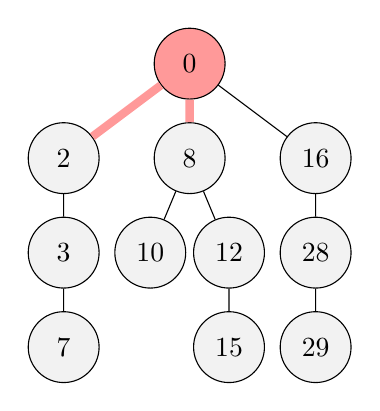
\begin{tikzpicture}
[level 1/.style={sibling distance=16mm, level distance=12mm},
level 2/.style={sibling distance=10mm, level distance=12mm}
]
\tikzset{every node/.style={shape=circle,draw,fill=black!5,minimum size=9mm}}
%\tikzset{every node/.style={shape=circle,
%                            font=\bfseries \Large,
%                            minimum size=3cm,
%                            scale=0.4
%                           }}
\node[fill=red!40] (root) {$0$}
    child {
        node {$2$}
        child {
            node {$3$}
            child {
                node {$7$}
            }
        };
    \path edge from parent[draw,line width=3pt,-,red!40];
    }
    child {
        node {$8$}
        child {
            node {$10$}
        }
        child {
            node {$12$}
            child {
                node {$15$}
            }
        };
    \path edge from parent[draw,line width=3pt,-,red!40];
    }
    child {
        node {$16$}
        child {
            node {$28$}
            child {
                node {$29$}
            }
        }
    }
    ;
\end{tikzpicture}
